\chapter{नाभिकीय भौतिकी}\label{ch:b3:nuclear-physics}

% Provenance (not for print): first half of the "physique subatomique"
% module common to the surveyed third-year curricula; particle physics
% follows in the next chapter. Deepens the high-school volume's
% radioactivity with SEMF, Gamow tunnelling and reactor physics.

विद्यालय के खंड ने कहानी की रूपरेखा बता दी थी: परमाणुओं में नाभिक
होते हैं; कुछ नाभिक भरभराकर गिर जाते हैं, और वह भी माइक्रोसेकंडों से
अरबों वर्षों तक फैली समय-सारणियों पर; और पदार्थ के ग्राम अपने भीतर
मेगाटन ऊर्जा छिपाए रहते हैं। यह अध्याय वर्ष 3 के औज़ारों के साथ नाभिक
को फिर से खोलता है। पाँच पदों वाला एक बूँद-प्रतिरूप सैकड़ों
न्यूक्लाइडों का बंधन प्रतिशत भर की परिशुद्धि से बता देता है; क्वांटम
सुरंगन --- यानी वर्ष 2 के खंड की रोधिका-समस्या, पदोन्नत --- समझा देता
है कि एक ही सूत्र $\alpha$-क्षय के जीवनकालों की पच्चीस कोटियों पर कैसे
फैल जाता है; और बंधन-ऊर्जा वक्र का लोहे पर बना वह चुप्पा अधिकतम पूरी
नाभिकीय प्रौद्योगिकी को दो खेमों में बाँट देता है: भारी को तोड़िए
(रिएक्टर) या हलके को जोड़िए (तारे, और किसी दिन बिजलीघर)। अध्याय किसी
रिएक्टर-कुंड के किनारे समाप्त होता है, जो चेरेनकोव नीले रंग में दहक
रहा है।

\section{नाभिक: एक संतृप्त बूँद}

\begin{definition}[न्यूक्लाइड, आकार, और घनत्व]\label{def:b3:nuclear-physics:nuclide}
\index{न्यूक्लाइड}\index{समस्थानिक}\index{नाभिकीय त्रिज्या}
कोई \emph{न्यूक्लाइड} $^{A}_{Z}\text{X}$ $Z$ प्रोटॉन और $N = A -
Z$ न्यूट्रॉन रखता है, जो \emph{प्रबल अन्योन्यक्रिया} से बँधे हैं: वह
तीव्र है (संपर्क पर कूलॉम का ${\sim}\qty{100}{}\times$), लघु-परास
(${\sim}\qty{1}{fm}$, केवल छूते पड़ोसी ही उसे अनुभव करते हैं), और
आवेश-अंधी (वह प्रोटॉन और न्यूट्रॉन, दोनों को एक-सा पकड़ती है)।
प्रकीर्णन प्रयोग हर नाभिक को वही एक नुस्खा देते हैं: त्रिज्या
\[
R = r_0A^{1/3} , \qquad r_0 \approx \qty{1.2}{fm} ,
\]
अतः आयतन $A$ की तरह बढ़ता है और घनत्व एक सार्वभौमिक
$\rho \approx \qty{2.3e17}{kg/m^3}$ है --- उसकी एक बूँद
टैंकरों के बेड़े जितनी भारी होगी, और
\cref{ch:b3:astrophysics} इसी घनत्व पर पूरे तारे से मिलेगा।
\emph{समस्थानिक} $Z$ साझा करते हैं पर $N$ में भिन्न होते हैं: वही
रसायन, भिन्न नाभिकीय नियति।
\end{definition}

\begin{proposition}[द्रव्यमान क्षति और बंधन ऊर्जा]\label{prop:b3:nuclear-physics:binding}
\index{द्रव्यमान क्षति}\index{बंधन ऊर्जा}\index{लोहे का शिखर}
कोई बद्ध नाभिक अपने अंगों से \emph{कम} भारी होता है; और
\cref{ch:b3:relativistic-dynamics} के अनुसार वह लापता द्रव्यमान ही
\omterm{prop:b3:nuclear-physics:binding}{बंधन ऊर्जा} है,
\[
B = \big(Zm_{\text{p}} + Nm_{\text{n}} - m_{\text{नाभिक}}\big)c^2 ,
\]
यानी प्रायः \emph{प्रति न्यूक्लिऑन} ${\sim}\qty{8}{MeV}$ --- रसायन का
दस लाख गुना। प्रति न्यूक्लिऑन आलेखित करने पर $B/A$ हलके नाभिकों में तेज़ी से चढ़ता है
(पृष्ठ-प्रभाव फीके पड़ जाते हैं), लोहा-56 के पास
$\approx\qty{8.8}{MeV}$ पर शिखर बनाता है, और फिर नीचे बहने लगता है,
क्योंकि कूलॉम प्रतिकर्षण, जो लंबी-परास का और असंतृप्त है, भारी
वालों पर कर लगाता है। दोनों ढलानें ऊर्जा की खानें हैं:
\emph{संलयन} बाईं ढलान चढ़ता है (सूर्य का कारोबार), और
\emph{विखंडन} दाईं ढलान से लुढ़कता है (रिएक्टर का) --- जबकि लोहा,
चोटी पर, दोनों के लिए नाभिकीय राख है।
\end{proposition}

\begin{omfigure}
\begin{tikzpicture}
  \begin{axis}[omaxis, axis x line=bottom, axis y line=left,
    width=11.2cm, height=6.2cm, xmin=0, xmax=250, ymin=0, ymax=10.3,
    xlabel={द्रव्यमान संख्या $A$}, ylabel={$B/A$ (\unit{MeV})},
    xlabel style={at={(axis description cs:0.5,-0.1)}, anchor=north},
    xtick={56,100,150,200,238}, ytick={2,4,6,8}, clip=false]
    \addplot[omDef, very thick, smooth] coordinates {
      (2,1.11) (3,2.7) (6,5.3) (9,6.46) (12,7.68) (16,7.98)
      (24,8.26) (40,8.55) (56,8.79) (75,8.7) (100,8.6)
      (125,8.45) (150,8.3) (175,8.1) (200,7.9) (220,7.75) (238,7.57)};
    \fill[omThm] (axis cs:4,7.07) circle (1.6pt);
    \draw[gray, thin] (axis cs:12.5,6.85) -- (axis cs:5.2,7.02);
    \node[omThm, font=\scriptsize, anchor=west] at (axis cs:13,6.8)
      {$^4$He};
    \fill[omThm] (axis cs:56,8.79) circle (1.6pt);
    \node[omThm, font=\scriptsize, anchor=south] at (axis cs:56,9.0)
      {$^{56}$Fe: चोटी};
    \fill[omThm] (axis cs:238,7.57) circle (1.6pt);
    \node[omThm, font=\scriptsize, anchor=south west] at (axis cs:225,7.85)
      {$^{238}$U};
    \draw[->, omExo, thick] (axis cs:14,4.0) -- (axis cs:40,6.4);
    \node[omExo, font=\scriptsize, anchor=west] at (axis cs:18,3.6)
      {संलयन चढ़ता है};
    \draw[->, omExo, thick] (axis cs:225,6.4) -- (axis cs:130,7.6);
    \node[omExo, font=\scriptsize, anchor=east] at (axis cs:242,5.9)
      {विखंडन लुढ़कता है};
  \end{axis}
\end{tikzpicture}

{\small बंधन-ऊर्जा वक्र --- शायद भौतिकी का सबसे परिणामदायी
आलेख। हलके नाभिक जुड़कर कमाते हैं, और भारी टूटकर;
प्रति किलोग्राम बाईं ढलान लगभग चार गुना बेहतर चुकाती है, और सूर्य
उसी पर बैठा है।}
\end{omfigure}

\begin{proposition}[अर्ध-आनुभविक द्रव्यमान सूत्र]\label{prop:b3:nuclear-physics:semf}
\index{अर्ध-आनुभविक द्रव्यमान सूत्र}\index{स्थायित्व की घाटी}
नाभिक का प्रतिरूप किसी आवेशित द्रव-बूँद से बनाइए, और पूरा वक्र
पाँच पदों से निकल आता है:
\[
B = a_{\text{V}}A - a_{\text{S}}A^{2/3}
- a_{\text{C}}\frac{Z^2}{A^{1/3}}
- a_{\text{A}}\frac{(A - 2Z)^2}{A} + \delta(A) ,
\]
जहाँ (\unit{MeV} में) $a_{\text{V}} = 15.8$ (हर न्यूक्लिऑन अपने
पड़ोसियों से बँधता है: आयतन), $a_{\text{S}} = 17.8$ (पृष्ठ के
न्यूक्लिऑन कम बँधते हैं: बूँद का ``पृष्ठ तनाव''), $a_{\text{C}} = 0.71$
(कूलॉम, वह लंबी-परास वाला तोड़फोड़िया), $a_{\text{A}} = 23.7$
(असममिति: \cref{ch:b3:quantum-statistics} के अनुसार प्रोटॉन और
न्यूट्रॉन दो अलग फ़र्मी सीढ़ियाँ भरते हैं, और सबसे सस्ता तब जब दोनों
बराबर भरी हों), और $\delta$ सम संख्याओं के लिए एक छोटा युग्मन-बोनस
(\cref{ch:b3:identical-particles})। स्थिर $A$ पर न्यूनतम करने से
\emph{\omterm{prop:b3:nuclear-physics:semf}{स्थायित्व की घाटी}} खिंच आती है: हलके नाभिकों के लिए $N \approx Z$,
जो न्यूट्रॉन-धनी की ओर मुड़ती जाती है ($N/Z \to 1.5$), क्योंकि कूलॉम
प्रोटॉनों को दंडित करता है --- और घाटी से बाहर के \omterm{def:b3:nuclear-physics:nuclide}{न्यूक्लाइड}
$\beta$ क्षय से उसमें लौट आते हैं।
\end{proposition}
\admitted

\begin{omfigure}
\begin{tikzpicture}
  \begin{axis}[omaxis, axis x line=bottom, axis y line=left,
    width=8.6cm, height=6.4cm, xmin=0, xmax=95, ymin=0, ymax=150,
    xlabel={प्रोटॉन $Z$}, ylabel={न्यूट्रॉन $N$},
    xlabel style={at={(axis description cs:0.5,-0.1)}, anchor=north},
    xtick={20,40,60,80}, ytick={50,100,150}, clip=true]
    \addplot[gray, dashed, domain=0:95] {x};
    \addplot[omDef, very thick, domain=1:92, samples=100]
      {x + 0.03*x^(5/3)};
    \node[gray, font=\scriptsize, anchor=north west] at
      (axis cs:78,74) {$N = Z$};
    \node[omDef, font=\scriptsize, anchor=north west, align=left] at
      (axis cs:48,125) {स्थायित्व\\की घाटी};
    \fill (axis cs:26,30) circle (1.5pt);
    \node[font=\scriptsize, anchor=north west] at (axis cs:26,29) {Fe};
    \fill (axis cs:92,146) circle (1.5pt);
    \node[font=\scriptsize, anchor=north west] at (axis cs:88,143) {U};
  \end{axis}
\end{tikzpicture}

{\small \omterm{prop:b3:nuclear-physics:semf}{स्थायित्व की घाटी}। हलके नाभिक अपनी दोनों
फ़र्मी सीढ़ियाँ संतुलित रखते हैं ($N = Z$); और भारी अपने कूलॉम बिल को
अतिरिक्त न्यूट्रॉनों से पतला करते हैं। घाटी के तल से बाहर पड़ा कोई
\omterm{def:b3:nuclear-physics:nuclide}{न्यूक्लाइड} $\beta$-क्षय करके उसकी ओर लौटता है --- और विखंडन-खंड, जो
उस रेखा से बहुत ऊपर जन्मते हैं, ठीक इसी कारण उग्र रूप से रेडियोसक्रिय
होते हैं।}
\end{omfigure}

\section{रेडियोसक्रियता, घड़ी के हिसाब से}

\begin{theorem}[क्षय का नियम]\label{thm:b3:nuclear-physics:decay}
\index{रेडियोसक्रिय क्षय का नियम}\index{अर्ध-आयु}\index{सक्रियता}
किसी अस्थायी नाभिक की न स्मृति होती है न बुढ़ापा: वह जितने भी सेकंड
जीता है, हर सेकंड उसी प्रायिकता $\lambda$ से क्षय करता है। $N$
नाभिकों के लिए $\dd N = -\lambda N\,\dd t$, अतः
\[
N(t) = N_0\,\eu^{-\lambda t} = N_0\,2^{-t/T_{1/2}} ,
\qquad T_{1/2} = \frac{\ln2}{\lambda} ,
\]
और \emph{सक्रियता} $\mathcal A = \lambda N$ (प्रति सेकंड क्षय,
\unit{Bq}) उसी चरघातांकी पर फीकी पड़ती है। अर्ध-आयु
माइक्रोसेकंडों से अरबों वर्षों तक चलती हैं; और
\cref{ch:b3:microcanonical-ensemble} की सांख्यिकी इसकी गारंटी देती है
कि जहाँ कोई एक नाभिक पूर्णतः अप्रत्याशित है, वहीं उनका एक मोल
किसी भी घड़ी से बेहतर चरघातांकी समय रखता है --- और यही
रेडियोमितीय काल-निर्धारण की नींव है।
\end{theorem}

\begin{proof}
प्रति सेकंड अचर प्रायिकता का अर्थ है $N(t + \dd t) = N(t)(1 -
\lambda\dd t)$; अब समाकलित कीजिए। और $N/N_0 = \tfrac12$ रखने पर
$T_{1/2}$ मिलता है।
\end{proof}

\begin{omfigure}
\begin{tikzpicture}
  \begin{axis}[omaxis, axis x line=bottom, axis y line=left,
    width=9.8cm, height=5.6cm, xmin=0, xmax=4.3, ymin=0, ymax=1.12,
    xlabel={$t/T_{1/2}$}, ylabel={$N/N_0$},
    xlabel style={at={(axis description cs:0.5,-0.1)}, anchor=north},
    xtick={1,2,3,4}, ytick={0.25,0.5,1},
    yticklabels={$\tfrac14$,$\tfrac12$,$1$}, clip=true]
    \addplot[omDef, very thick, domain=0:4.3, samples=150]
      {exp(-0.6931*x)};
    \draw[gray, dashed] (axis cs:0,0.5) -| (axis cs:1,0);
    \draw[gray, dashed] (axis cs:0,0.25) -| (axis cs:2,0);
    \node[font=\scriptsize, anchor=south west, align=left] at
      (axis cs:2.3,0.55) {हर अर्ध-आयु\\गिनती आधी कर देती है};
  \end{axis}
\end{tikzpicture}

{\small चरघातांकी क्षय: व्यक्ति स्मृतिहीन, जनसंख्या समयनिष्ठ।
दो अर्ध-आयु एक चौथाई छोड़ जाती हैं; और दस एक
हज़ारवाँ --- वही मापपट्टी, जिससे भौतिकीविद् कोयला, हिमनद और पृथ्वी,
सबकी आयु निकालते हैं।}
\end{omfigure}

\begin{remark}[नाभिक से बाहर के तीन दरवाज़े]\label{rem:b3:nuclear-physics:modes}
\index{अल्फ़ा क्षय}\index{बीटा क्षय}\index{गामा क्षय}\index{गामो प्रतिरूप}
$\boldsymbol\alpha$: कोई भारी नाभिक $^4$He का गुच्छा उत्सर्जित करता
है। चिरसम्मत ढंग से यह असंभव है --- कूलॉम रोधिका \qty{25}{MeV} तक
चढ़ती है और वह $\alpha$ \qty{5}{}--\qty{9}{MeV} लेकर निकलता है ---
पर यह \emph{सुरंगन} से होता है (वर्ष 2 के खंड की रोधिका, मुड़ी हुई):
गामो की चरघातांकी संवेदनशीलता ऊर्जा के दो गुने को जीवनकाल की बीस
कोटियों में बदल देती है, और यही ठीक गाइगर--नटॉल
प्रतिरूप है (\cref{exo:b3:nuclear-physics:8})।
$\boldsymbol\beta$: कोई न्यूट्रॉन प्रोटॉन बन जाता है (या उलटा), और
एक इलेक्ट्रॉन (या पॉज़िट्रॉन) तथा एक न्यूट्रिनो उत्सर्जित करता है ---
यानी \emph{दुर्बल अन्योन्यक्रिया} काम पर, यानी घाटी लौटाने वाला बल;
और न्यूट्रिनो की कहानी \cref{ch:b3:particle-physics} की प्रतीक्षा
करती है।
$\boldsymbol\gamma$: कोई उत्तेजित नाभिक \unit{MeV} के फ़ोटॉन झाड़ देता
है, जो \cref{ch:b3:hydrogen-atom} की वर्णक्रमीय रेखाओं का नाभिकीय
समरूप है। क्षय तब तक शृंखला में चलते हैं जब तक घाटी का तल न आ जाए:
यूरेनियम की सीढ़ी चौदह पायदान बाद स्थायी सीसे पर समाप्त होती है।
\end{remark}

\section{ढलानों से नीचे: विखंडन और संलयन}

\begin{proposition}[विखंडन और शृंखला अभिक्रिया]\label{prop:b3:nuclear-physics:fission}
\index{विखंडन}\index{शृंखला अभिक्रिया}\index{क्रांतिक द्रव्यमान}
$^{235}$U द्वारा सोखा गया कोई धीमा न्यूट्रॉन एक डगमगाती बूँद बना देता
है, जो टूट जाती है: दो मध्य-द्रव्यमान खंड, दो-तीन ताज़े न्यूट्रॉन, और
$\approx\qty{200}{MeV}$ --- यानी यूरेनियम की \qty{7.6}{MeV} और खंडों
की \qty{8.5}{MeV} के बीच का $B/A$ अंतर, गुणा 235।
मुक्त हुए न्यूट्रॉन और नाभिकों का विखंडन कर सकते हैं: गुणन गुणक
$k$ (एक पीढ़ी बाद प्रति न्यूट्रॉन कितने न्यूट्रॉन) के साथ कोई
जनसंख्या $k^n$ की तरह बढ़ती है --- अवक्रांतिक ($k < 1$) बुझ जाती है,
क्रांतिक ($k = 1$) स्थिर रहती है, और अतिक्रांतिक फट पड़ती है।
कोई रिएक्टर न्यूट्रॉनों को धीमी चालों तक मंदित करता है (विखंडन का
पसंदीदा भोजन), उन 0.7\,\% न्यूट्रॉनों पर टिकता है जो खंडों के क्षय से
\emph{सेकंडों} देर से आते हैं --- वही देरी, जो $k \approx 1$ को
मनुष्य के लिए समायोज्य बना देती है --- और नियंत्रण छड़ों को अतिरेक
खाने देता है (\cref{pb:b3:nuclear-physics:1})।
\end{proposition}
\admitted

\begin{omfigure}
\begin{tikzpicture}[scale=1.0]
  % stage 1: nucleus + neutron
  \draw[->, thick] (-1.3,0) -- (-0.55,0);
  \fill[gray] (-1.55,0) circle (2.6pt);
  \node[font=\scriptsize, anchor=south] at (-1.55,0.12) {n};
  \draw[omDef, fill=omDef!15, thick] (0.35,0) circle (0.62);
  \node[omDef, font=\scriptsize] at (0.35,0) {$^{235}$U};
  % arrow
  \draw[->, thick] (1.35,0) -- (2.05,0);
  % stage 2: deformed drop (peanut)
  \draw[omDef, fill=omDef!15, thick, rotate around={0:(3.1,0)}]
    (3.1,0) ellipse (0.85 and 0.42);
  \draw[omDef!60, dashed] (3.1,-0.5) -- (3.1,0.5);
  % arrow
  \draw[->, thick] (4.3,0) -- (5.0,0);
  % stage 3: fragments + neutrons
  \draw[omThm, fill=omThm!12, thick] (5.9,0.55) circle (0.42);
  \draw[omThm, fill=omThm!12, thick] (5.9,-0.55) circle (0.42);
  \node[omThm, font=\tiny] at (5.9,0.55) {Ba};
  \node[omThm, font=\tiny] at (5.9,-0.55) {Kr};
  \foreach \ang in {15,-8,40}{
    \fill[gray] ({6.7+0.35*cos(\ang)},{0.3*sin(\ang)}) circle (2.2pt);
    \draw[->, gray] ({6.95+0.35*cos(\ang)},{0.32*sin(\ang)}) --
      ({7.55+0.35*cos(\ang)},{0.42*sin(\ang)});}
  \node[font=\scriptsize, anchor=west, align=left] at (8.05,0)
    {2--3 न्यूट्रॉन\\$+\ \qty{200}{MeV}$};
\end{tikzpicture}

{\small द्रव-बूँद विखंडन: कोई धीमा न्यूट्रॉन $^{235}$U को
डगमगा देता है; उस विरूपित बूँद का कूलॉम प्रतिकर्षण उसके पृष्ठ तनाव
पर भारी पड़ता है, और वह न्यूट्रॉन-धनी खंडों में चिर जाती है, साथ में
वे फ़ालतू न्यूट्रॉन भी जो कोई शृंखला संभव बनाते हैं।}
\end{omfigure}

\begin{remark}[संलयन: कठिन, पर बेहतर ढलान]\label{rem:b3:nuclear-physics:fusion}
\index{संलयन}
हलके नाभिकों को जोड़ना भारी नाभिकों को तोड़ने से प्रति किलोग्राम
$\sim4\times$ अधिक चुकाता है, और उसमें कोई दीर्घजीवी खंड भी नहीं ---
पर दोनों अभिकारक, जो धन आवेशित हैं, अपनी परस्पर कूलॉम रोधिका में
सुरंग बनाकर निकलें, इसके लिए $10^7$--$10^8\,\unit{K}$ के ताप चाहिए
(\cref{exo:b3:nuclear-physics:11})। तारे इसे विशाल होकर कर लेते हैं
(\cref{ch:b3:astrophysics}: सूर्य हर सेकंड \qty{600}{} लाख
टन हाइड्रोजन को हीलियम में बदलता है); और प्रयोगशालाएँ इसे
चुंबकीय बोतलों में बंद प्लाज़्मा से करती हैं, जिनका ऊर्जा-बहीखाता
अब तक अपनी बराबरी की महत्वाकांक्षाओं से कुछ पीछे ही है।
\end{remark}

\begin{omfigure}
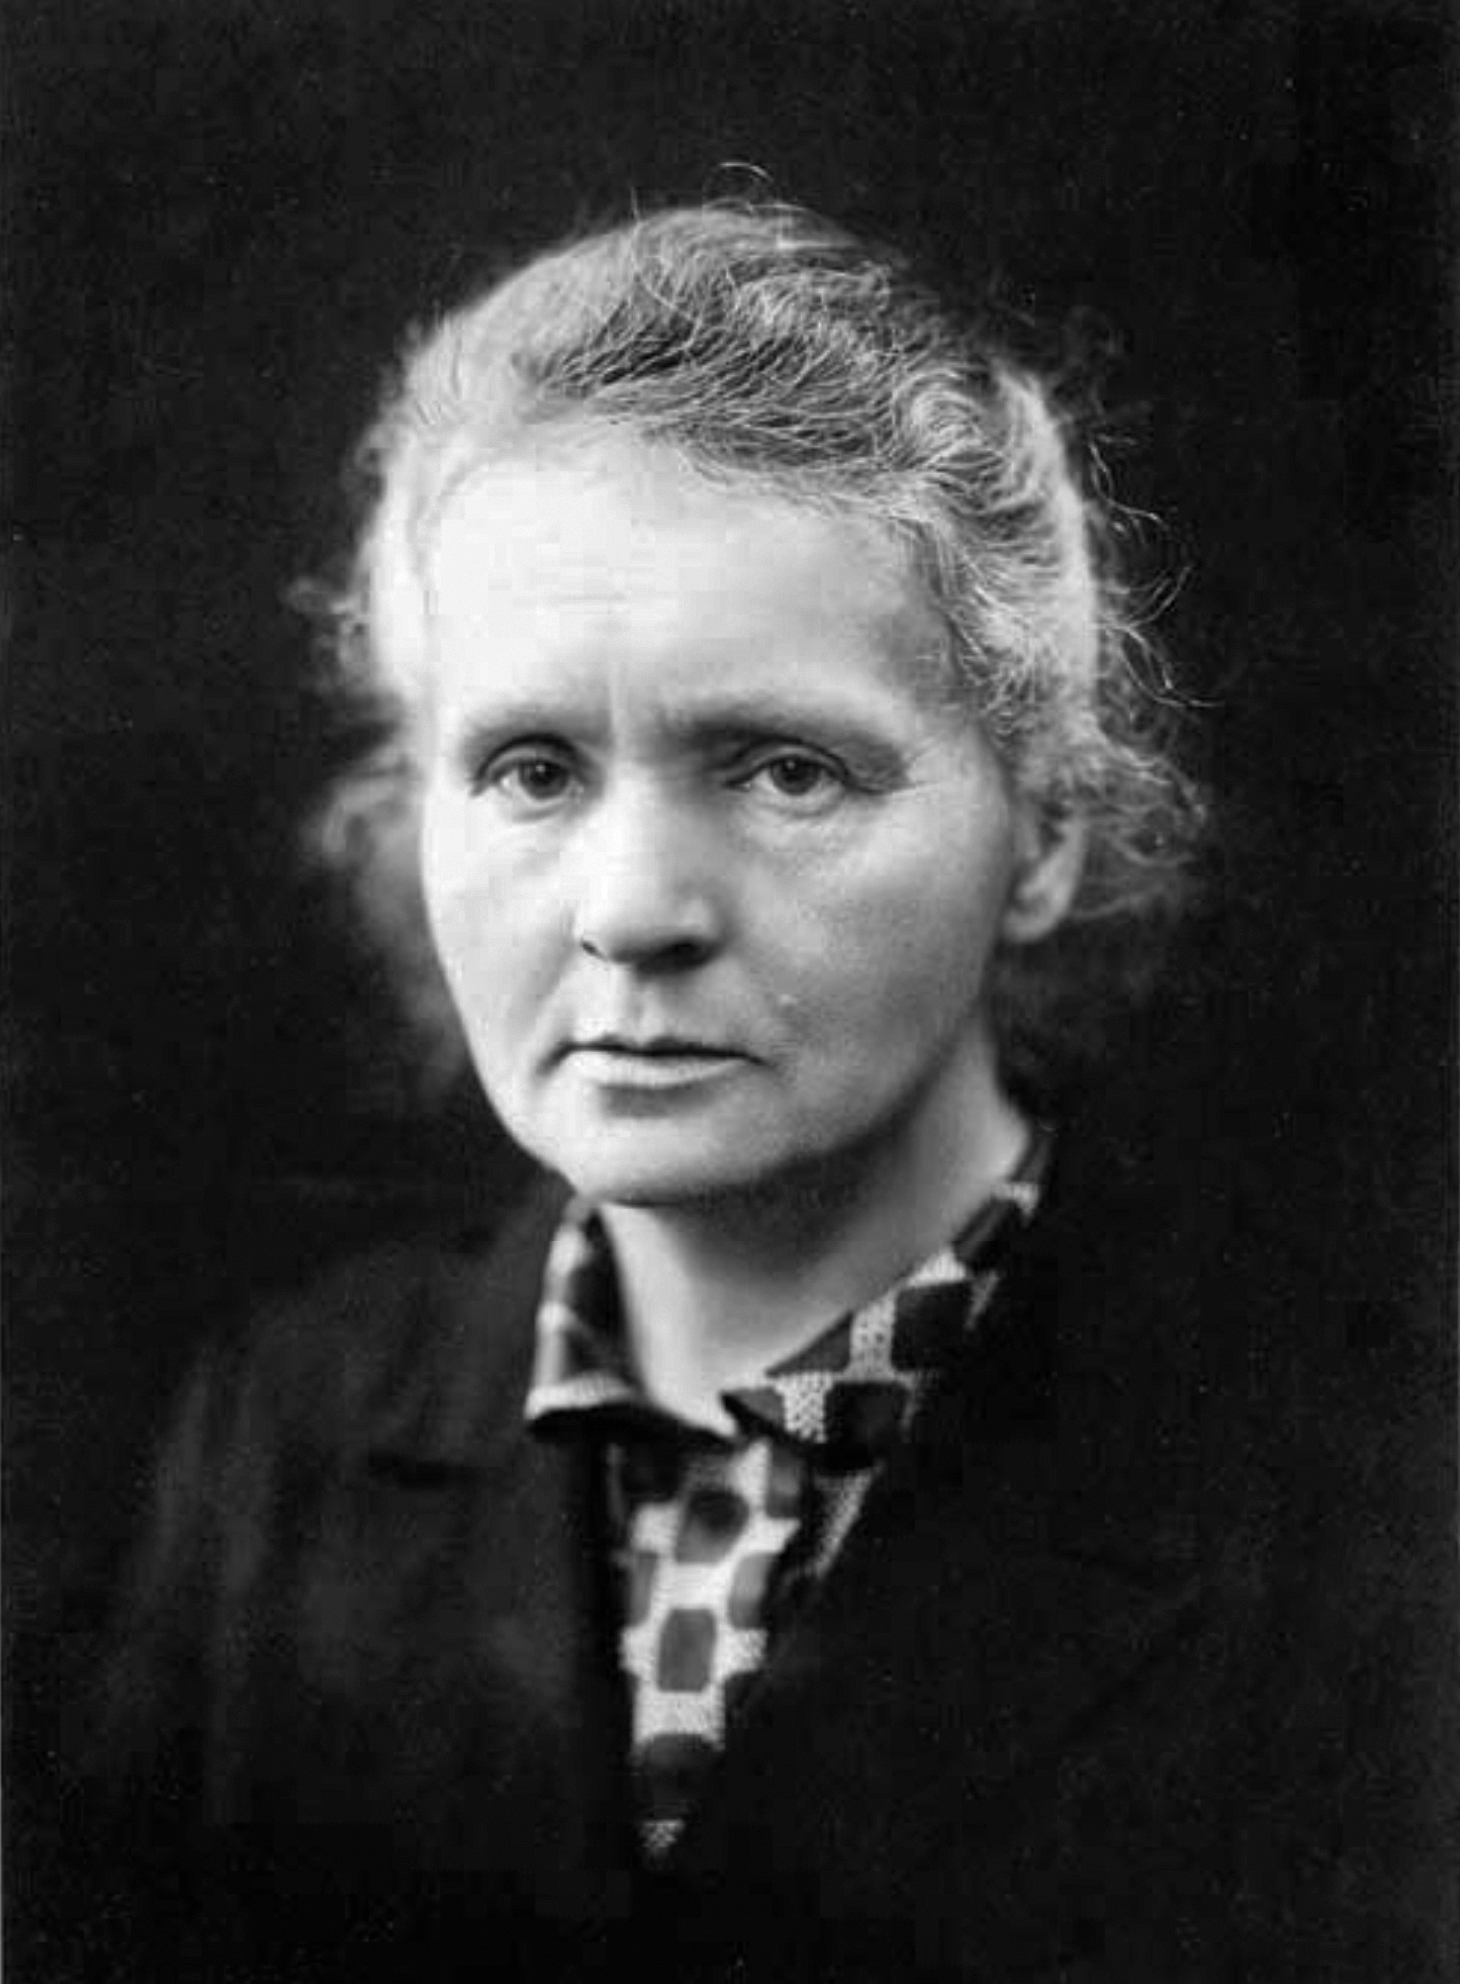
\includegraphics[width=0.34\linewidth]{images/book5/photo-marie-curie.jpg}

{\small मारी क्यूरी (छायाचित्र: आँरी मानुएल, लगभग 1920, सार्वजनिक डोमेन): इस अध्याय का विषय खोलने के लिए दो बार की नोबेल विजेता --- \cref{exo:b3:nuclear-physics:4} वाला रेडियम का ग्राम उन्हीं का था।}
\end{omfigure}

\section{अभ्यास}

\begin{exercise}[$\star$]\label{exo:b3:nuclear-physics:1}
हिसाब-किताब। (क) $Z$, $N$, $A$ दीजिए, $^{12}$C, $^{14}$C,
$^{235}$U, $^{238}$U के लिए। (ख) कौन-से जोड़े
\omterm{def:b3:nuclear-physics:nuclide}{समस्थानिक} हैं? (ग) \omterm{def:b3:nuclear-physics:nuclide}{समस्थानिक} रसायन तो साझा करते हैं, पर नाभिकीय
स्थायित्व क्यों नहीं? (घ) $^{14}$C
और $^{14}$N $A = 14$ साझा करते हैं: ऐसे \omterm{def:b3:nuclear-physics:nuclide}{न्यूक्लाइड} क्या कहलाते हैं,
और कौन-सा क्षय उन्हें जोड़ता है?
\end{exercise}

\begin{exercise}[$\star$]\label{exo:b3:nuclear-physics:2}
सार्वभौमिक घनत्व। (क) $R = r_0A^{1/3}$ से दिखाइए कि
नाभिकीय घनत्व $A$ से स्वतंत्र है, और उसका मान निकालिए। (ख)
नाभिकीय पदार्थ की एक चम्मच (\qty{5}{mL}) का द्रव्यमान निकालिए।
(ग) किसी परमाणु के आयतन का कितना अंश उसका नाभिक भरता है (लीजिए
$R_{\text{परमाणु}} = \qty{1e-10}{m}$, $A = 60$)? (घ) स्वयं
$A^{1/3}$ नियम प्रबल बल की परास के बारे में क्या कहता है?
\end{exercise}

\begin{exercise}[$\star$]\label{exo:b3:nuclear-physics:3}
गोंद को तौलना। नाभिकीय द्रव्यमान: $m_{\text{p}} =
\qty{1.007276}{u}$, $m_{\text{n}} = \qty{1.008665}{u}$,
$m(^4\text{He}) = \qty{4.001506}{u}$;
$\qty{1}{u}\,c^2 = \qty{931.5}{MeV}$। (क) $^4$He की \omterm{thm:b3:relativistic-dynamics:emc2}{द्रव्यमान
क्षति} और \omterm{prop:b3:nuclear-physics:binding}{बंधन ऊर्जा} निकालिए। (ख) $B/A$ दीजिए। (ग) $B$ की तुलना
\cref{ch:b3:hydrogen-atom} की \qty{13.6}{eV} से कीजिए: नाभिकीय और
परमाणविक गोंद के बीच कितनी कोटियाँ हैं? (घ)
$^4$He का असाधारण बंधन (चित्र वाली शलाका) उसे $\alpha$ क्षय की मुद्रा
क्यों बना देता है?
\end{exercise}

\begin{exercise}[$\star$]\label{exo:b3:nuclear-physics:4}
पहला क्यूरी। रेडियम-226: $T_{1/2} = 1600$ वर्ष, मोलर द्रव्यमान
\qty{226}{g/mol}। एक ग्राम के लिए: (क) नाभिक गिनिए; (ख)
$\lambda$ निकालिए; (ग) सक्रियता निकालिए और ऐतिहासिक इकाई
$1\,\text{Ci} = \qty{3.7e10}{Bq}$ से तुलिए (जो ठीक इसी
ग्राम से परिभाषित हुई थी); (घ) 4800 वर्ष बाद उस ग्राम का कितना बचता है?
\end{exercise}

\begin{exercise}[$\star\star$]\label{exo:b3:nuclear-physics:5}
सूत्र काम पर। $a_{\text{V}} = 15.75$,
$a_{\text{S}} = 17.8$, $a_{\text{C}} = 0.711$,
$a_{\text{A}} = 23.7$ (\unit{MeV}) और सम--सम नाभिकों के लिए युग्मन
$+12/\sqrt A$ के साथ: (क) $B$ के चारों मुख्य पद निकालिए,
$^{56}$Fe ($Z = 26$) के लिए। (ख) (युग्मन सहित) जोड़िए और
$B/A$ की तुलना मापे गए \qty{8.79}{MeV} से कीजिए। (ग) कौन-से दो
पद सबसे कड़ी लड़ाई लड़ते हैं, और उनका संतुलन क्या तय करता है? (घ)
अकेले कूलॉम पद को $A$ से \emph{तेज़} क्यों बढ़ना पड़ता है?
\end{exercise}

\begin{exercise}[$\star\star$]\label{exo:b3:nuclear-physics:6}
घाटी का तल। (क) केवल $Z$-निर्भर पद रखकर स्थिर $A$ पर
द्रव्यमान न्यूनतम कीजिए और व्युत्पन्न कीजिए
$Z^* = \dfrac{A/2}{1 + a_{\text{C}}A^{2/3}/4a_{\text{A}}}$। (ख)
$A = 101$ के लिए मान निकालिए और रुथेनियम ($Z = 44$) से तुलिए।
(ग) दिखाइए कि हलके-$A$ की सीमा $Z^* = A/2$ है और उसे दोनों फ़र्मी
सीढ़ियों से समझाइए। (घ) किसी विखंडन-खंड का $A = 95$,
$Z = 36$ है: वह घाटी से कितना दूर है, और उसके बाद क्षयों का कौन-सा
क्रम आता है?
\end{exercise}

\begin{exercise}[$\star\star$]\label{exo:b3:nuclear-physics:7}
रेडियोकार्बन। जीवित पदार्थ अपने $^{14}$C
($T_{1/2} = 5730$ वर्ष) को प्रति $10^{12}$ कार्बन पर 1 परमाणु पर
भरा रखता है; और मृत्यु उस भरपाई को रोक देती है। (क) कोयले का कोई
नमूना जीवित सक्रियता का 30\,\% दिखाता है: वह आग कितनी पुरानी है? (ख)
जीवित कार्बन का एक ग्राम: उसकी $^{14}$C सक्रियता निकालिए
(अपेक्षित $\approx\qty{0.23}{Bq}$)। (ग) यह विधि
$\sim\qty{50000}{}$ वर्ष से आगे बेकार क्यों है? (घ) और चट्टानों की
आयु निकालने के लिए बेकार क्यों (कौन-सी घड़ियाँ कमान लेती हैं)?
\end{exercise}

\begin{exercise}[$\star\star$]\label{exo:b3:nuclear-physics:8}
गामो की चट्टान। पोलोनियम-212 \qty{8.78}{MeV} का $\alpha$ उत्सर्जित
करता है; और उसकी रोधिका $\approx\qty{26}{MeV}$ तक चढ़ती है। (क)
दिखाइए कि चिरसम्मत निकास असंभव है, और चिरसम्मत प्रवेश भी --- फिर भी
वह \qty{0.3}{\micro s} में क्षय कर देता है। (ख) यूरेनियम-238 का
$\alpha$ \qty{4.2}{MeV} ढोता है और उसकी अर्ध-आयु $4.5\times10^9$ वर्ष
है: दोनों क्षय-नियतांकों का अनुपात निकालिए। (ग)
सुरंगन-चरघातांकी से समझाइए कि ऊर्जा में दो गुना दर में
$\sim10^{24}$ कैसे खरीद लेता है। (घ) वही भौतिकी
सूर्य के क्रोड की ताप-आवश्यकता क्यों तय करती है?
\end{exercise}

\begin{exercise}[$\star\star$]\label{exo:b3:nuclear-physics:9}
बीस करोड़ इलेक्ट्रॉन-वोल्ट। (क) प्रति विखंडन $\qty{200}{MeV}$ को
$B/A$ वक्र से उचित ठहराइए। (ख) पूरी तरह विखंडित
$^{235}$U के एक किलोग्राम में ऊर्जा निकालिए, जूल में और तेल-तुल्य
टनों में (\qty{42}{GJ/t})। (ग) 33\,\% दक्षता पर कोई
\qty{1}{GW_e} बिजलीघर: प्रति वर्ष कितने किलोग्राम $^{235}$U? (घ)
न्यूट्रॉन नहीं, बल्कि खंड ही अधिकांश
\qty{200}{MeV} क्यों ढोते हैं, और वह तुरंत किस रूप में बदल जाती है?
\end{exercise}

\begin{exercise}[$\star\star\star$]\label{exo:b3:nuclear-physics:10}
$k$ को साधना। किसी रिएक्टर में तात्कालिक न्यूट्रॉन $\ell
\approx \qty{e-4}{s}$ में प्रजनन करते हैं। (क) केवल तात्कालिक
न्यूट्रॉनों पर $k = 1.001$ के साथ एक सेकंड में शक्ति का गुणन निकालिए
--- और यांत्रिक नियंत्रण पर फ़ैसला भी। (ख) कोई अंश $\beta =
0.7\,\%$ न्यूट्रॉनों का $\sim\qty{10}{s}$ तक \emph{विलंबित} रहता है:
समझाइए कि $k - 1 < \beta$ के लिए उस शृंखला की प्रभावी घड़ी
सेकंडों की क्यों हो जाती है। (ग) प्रभावी पीढ़ी-काल
$\sim\qty{0.1}{s}$ के साथ वही एक-सेकंड वाला गुणन निकालिए। (घ) एक
वाक्य में बताइए कि जब चेर्नोबिल का रिएक्टर तात्कालिक-अतिक्रांतिक हो
गया तब उसके संचालकों ने क्या खो दिया।
\end{exercise}

\begin{exercise}[$\star\star\star$]\label{exo:b3:nuclear-physics:11}
सूर्य का अंकगणित। कुल मिलाकर $4\,^1\text{H} \to {}^4\text{He}$
द्रव्यमान का \qty{0.71}{\percent} ऊर्जा में बदल देता है
(\qty{26.7}{MeV}, न्यूट्रिनो सहित)। (क) $L_\odot =
\qty{3.8e26}{W}$ से प्रति सेकंड बदला गया द्रव्यमान निकालिए, और
प्रति सेकंड खपा हुआ हाइड्रोजन भी। (ख) $\qty{2e30}{kg}$ के सूर्य
में से दसवाँ भाग जलने योग्य क्रोड-हाइड्रोजन लेकर (हाइड्रोजन-अंश
$\approx0.75$ मानिए): उसका जीवनकाल आकलिए। (ग)
\qty{1.5e7}{K} पर दो प्रोटॉन: $k_{\text{B}}T$ की तुलना
\qty{1}{fm} पर उनकी कूलॉम रोधिका से कीजिए और तय कीजिए कि पार कौन
करता है (\cref{exo:b3:nuclear-physics:8})। (घ) विखंडन के विपरीत
संलयन लगभग कोई रेडियोसक्रिय राख क्यों नहीं छोड़ता?
\end{exercise}

\begin{exercise}[$\star\star\star$]\label{exo:b3:nuclear-physics:12}
नाभिकीय चिकित्सा। (क) टेक्नीशियम-99m ($T_{1/2} = \qty{6}{h}$,
\qty{140}{keV} का $\gamma$) चिकित्सा का मज़दूर है: किसी इंजेक्ट की
गई \qty{500}{MBq} के पीछे नाभिकों की संख्या और
उनका द्रव्यमान निकालिए। (ख) समझाइए कि छह \emph{घंटे} की अर्ध-आयु और
कोई शुद्ध $\gamma$, दोनों ही किसी निदान की ठीक-ठीक ज़रूरत क्यों हैं। (ग)
PET: $^{18}$F का कोई पॉज़िट्रॉन किसी इलेक्ट्रॉन से नष्ट होता है ---
\cref{ch:b3:relativistic-dynamics} से दोनों फ़ोटॉनों की ऊर्जा और
ज्यामिति दीजिए, और इस तरह उस संसूचक का सिद्धांत भी।
(घ) विकिरण-चिकित्सा किसी अर्बुद को \qty{2}{Gy} (\unit{J/kg}) देती है:
उस ऊर्जा की तुलना गरम पानी के एक घूँट से कीजिए, और उन जूलों की
निर्दोषता को आयनन की घातकता से मिलाइए।
\end{exercise}

\begin{omfigure}
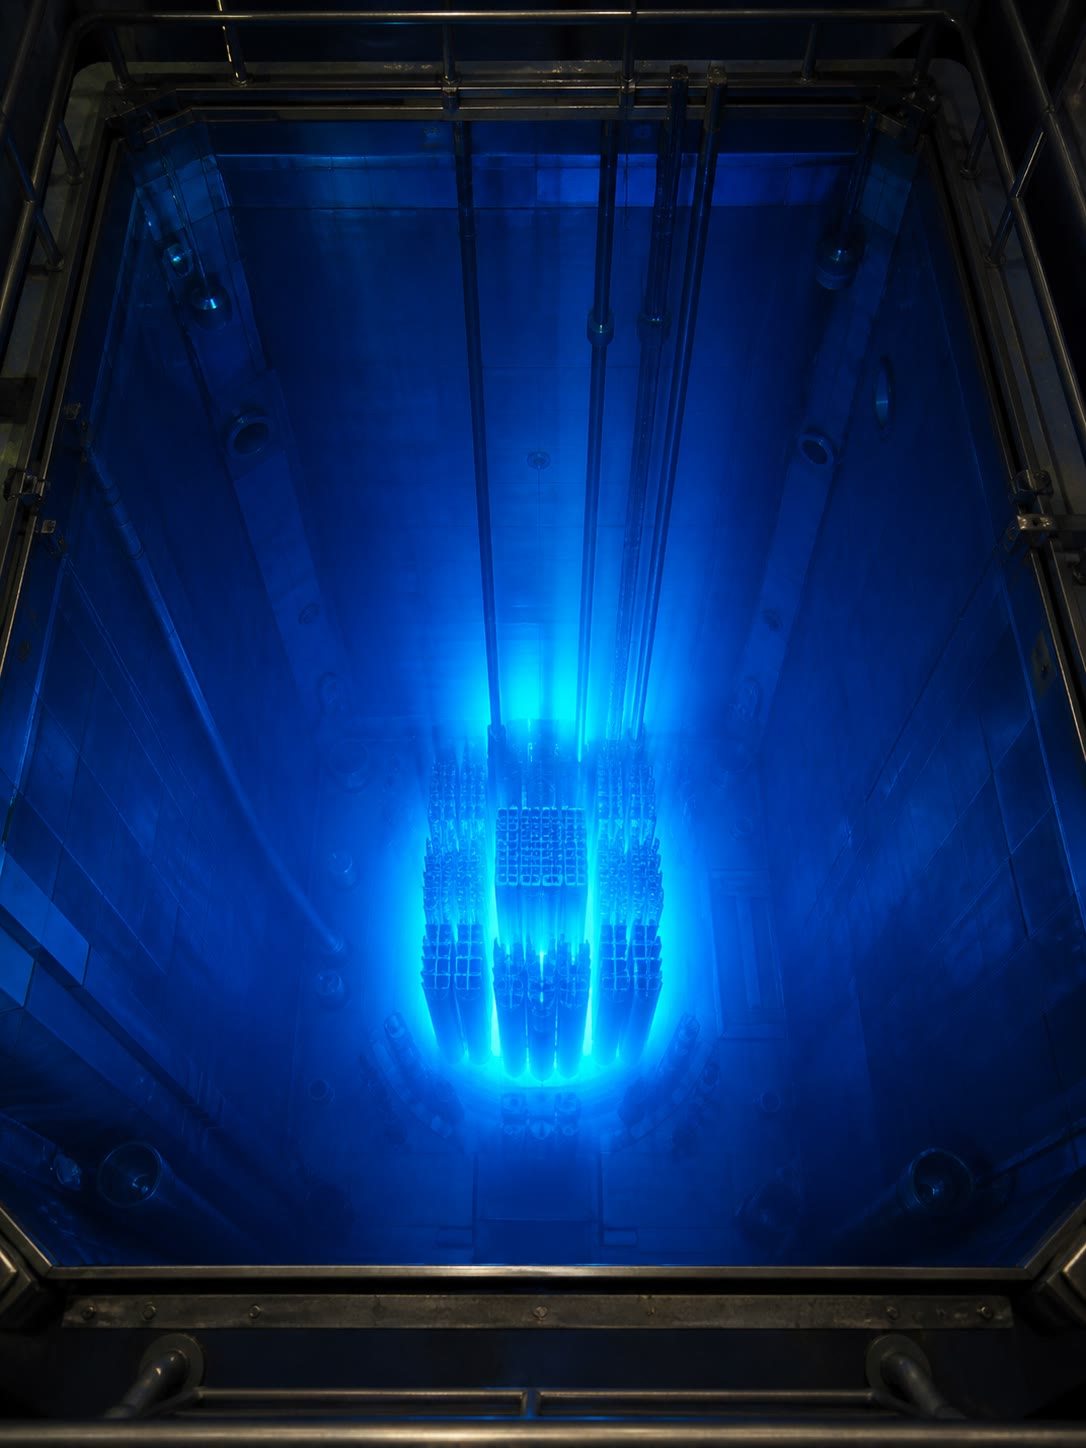
\includegraphics[width=0.45\linewidth]{images/book5/ai/b5-21-cherenkov-pool.jpg}

{\small सप्ताहांत समस्या का रिएक्टर-कुंड: खंडों के $\beta$ इलेक्ट्रॉन पानी में प्रकाश से आगे निकलकर क्रोड को चेरेनकोव नीले रंग में लपेट देते हैं --- यानी परिरक्षण, दिखाई देता हुआ काम पर।}
\end{omfigure}

\section{समस्या: शोध-रिएक्टर पर खुला दिवस}

\begin{problem}\label{pb:b3:nuclear-physics:1}
\emph{शोध-रिएक्टर पर खुला दिवस।} राष्ट्रीय प्रयोगशाला अपना
\qty{20}{MW} का कुंड-प्रकार शोध-रिएक्टर आगंतुकों के लिए खोलती है, और
आप बातें बनाकर बालकनी तक पहुँच गए हैं: नीचे, आठ
मीटर स्वच्छ पानी से होकर, वह क्रोड एक अलौकिक नीले रंग में दहक रहा है।
मार्गदर्शक --- सेवानिवृत्त होते एक रिएक्टर-भौतिकीविद् --- ने आपको
अंकगणित करने की छूट दे दी है।

\medskip\noindent\textbf{भाग I --- ऊर्जा का बहीखाता।}

\begin{enumerate}
  \item $^{235}$U का हर विखंडन लगभग \qty{200}{MeV} मुक्त करता है।
        उसे जूल में बदलिए, और \qty{20}{MW} बनाए रखने वाले प्रति
        सेकंड विखंडन निकालिए।
  \item उसे प्रति दिन खपे $^{235}$U के ग्रामों में बदलिए।
  \item वही \qty{20}{MW} कोयले से (\qty{30}{MJ/kg}): प्रति दिन
        कितने टन? द्रव्यमान-अनुपात बनाइए और उसे इस अध्याय तथा रसायन
        के \unit{MeV}-बनाम-\unit{eV} पैमानों से
        जोड़िए।
  \item खंड प्रति न्यूक्लिऑन $\sim\qty{8.5}{MeV}$ बंधन पर जन्मते
        हैं और यूरेनियम \qty{7.6}{MeV} पर: सत्यापित कीजिए कि
        $235\times0.9 \approx \qty{200}{MeV}$ संगत है।
  \item वे खंड अपने जन्मस्थान के माइक्रोमीटरों भीतर ही रुक जाते हैं।
        उनकी \qty{200}{MeV} किसमें बदलती है, और किस समय-पैमाने पर वह
        शीतलक पानी तक पहुँचती है?
  \item वे खंड (उदाहरण के लिए $A = 95$, $Z = 36$) अनिवार्यतः
        रेडियोसक्रिय क्यों हैं? \omterm{prop:b3:nuclear-physics:semf}{स्थायित्व की घाटी} काम में लीजिए।
\end{enumerate}

\medskip\noindent\textbf{भाग II --- $k = 1$ बनाए रखना।}

\begin{enumerate}[resume]
  \item गुणन गुणक $k$ परिभाषित कीजिए और बताइए कि न्यूट्रॉन-जनसंख्या
        के लिए $k = 0.999$, $1.000$, $1.001$ का क्या अर्थ है।
  \item कुंड का पानी मंदन करता है। दो वाक्यों में समझाइए कि
        न्यूट्रॉनों को तापीय चालों तक धीमा करना $^{235}$U का विखंडन
        क्यों \emph{आसान} करता है, और हाइड्रोजन सबसे अच्छा मंदक
        क्यों है (वर्ष 1 के खंड के प्रत्यास्थ संघट्ट याद कीजिए)।
  \item नियंत्रण छड़ें बोरॉन-इस्पात की हैं। बोरॉन क्या करता है, और
        छड़ों को उठाना-गिराना $k$ को कैसे साधता है?
  \item केवल तात्कालिक न्यूट्रॉनों ($\ell = \qty{e-4}{s}$) और
        $k = 1.0005$ के साथ एक सेकंड में शक्ति की वृद्धि निकालिए
        और निष्कर्ष निकालिए।
  \item 0.7\,\% विलंबित न्यूट्रॉन प्रभावी पीढ़ी-काल को
        $\sim\qty{0.1}{s}$ तक खींच देते हैं: फिर से निकालिए, और वह
        अभिकल्पना-नियम बताइए जो $k - 1$ को विलंबित अंश से सुरक्षित
        नीचे रखता है।
  \item वह पानी शीतलक भी है। उसकी अंतर्निहित सुरक्षा-विशेषता
        समझाइए: यदि पानी उबलकर उड़ जाए तो मंदन का --- और इस तरह
        $k$ का --- क्या होता है?
  \item बंद करने के बाद भी उस रिएक्टर को आपात शीतलन क्यों चाहिए?
        (उस ऊष्मा-स्रोत का नाम लीजिए जिसे नियंत्रण छड़ें छू भी नहीं
        सकतीं।)
\end{enumerate}

\medskip\noindent\textbf{भाग III --- नीली रोशनी।}

\begin{enumerate}[resume]
  \item वह चमक चेरेनकोव विकिरण है: पानी में प्रकाश की चाल
        $c/n$ है, जहाँ $n = 1.33$। उसे उत्सर्जित करने के लिए किसी
        आवेशित कण को क्या करना पड़ता है?
  \item देहली-चाल निकालिए, और
        \cref{ch:b3:relativistic-dynamics} की मदद से किसी इलेक्ट्रॉन
        के लिए देहली-गतिज ऊर्जा भी।
  \item रिएक्टर के कौन-से कण योग्य ठहरते हैं? विखंडन-खंड से लेकर
        पानी में तेज़ $\beta$ इलेक्ट्रॉन तक की शृंखला बताइए।
  \item उस वर्णक्रम की तीव्रता छोटी तरंगदैर्घ्यों की ओर बढ़ती है:
        वह कुंड लाल के बजाय नीला क्यों दहकता है?
  \item मार्गदर्शक कहता है: ``वह चमक \emph{ही} परिरक्षण का काम करना
        है।'' समझाइए --- पानी के आठ मीटर क्रोड के विकिरण का क्या
        करते हैं, और वह बालकनी मोटे तौर पर सुरक्षित क्यों है?
  \item बंद करने के बाद वह नीलापन मिनटों में मंद पड़ता है, पर दिनों
        तक लुप्त नहीं होता। भाग I के प्रश्न 6 से जोड़िए।
\end{enumerate}

\medskip\noindent\textbf{भाग IV --- रिएक्टर है किसलिए।}

\begin{enumerate}[resume]
  \item इस रिएक्टर का रोज़ का काम मॉलिब्डेनम-99
        ($T_{1/2} = \qty{66}{h}$) बनाना है, जो चिकित्सा के
        टेक्नीशियम-99m का जनक है। दुनिया के अस्पतालों को हर सप्ताह
        फिर से आपूर्ति क्यों चाहिए, और कोई गोदाम उसे जमा क्यों नहीं
        कर सकता?
  \item \qty{100}{GBq} की मॉलिब्डेनम-99 खेप सोमवार को निकलती है;
        और अस्पताल शुक्रवार को (96 घंटे बाद) टेक्नीशियम-99m का
        निक्षालन करता है। जनक की कितनी सक्रियता बची रहती है?
  \item क्रोड से निकलते न्यूट्रॉन पुंज
        \cref{ch:b3:crystalline-solids} के विवर्तन-उपकरणों को भी
        खिलाते हैं: रिएक्टर के न्यूट्रॉन, एक बार तापीय हो जाने पर,
        सही तरंगदैर्घ्य के साथ ही क्यों जन्मते हैं?
  \item मार्गदर्शक की विदाई-समस्या: कोई ईंधन-तत्त्व भेजे जाने से
        पहले पाँच वर्ष उस कुंड में बिताता है। खंडों की अर्ध-आयुओं के
        मिश्रण से उस तर्क को समझाइए --- कुंड में बिताए पाँच वर्षों
        ने क्या खरीदा?
  \item बंद करने के एक घंटे बाद क्षय-ऊष्मा आकलिए
        (\qty{20}{MW} का $\approx1\,\%$) और उसकी तुलना किसी घर के
        बिजली-हीटर से कीजिए: क्या निष्क्रिय कुंड-शीतलन विश्वसनीय है?
  \item बहीखाता चार पंक्तियों में बंद कीजिए: $B/A$ प्रति विभाजन
        \qty{200}{MeV} चुकाता है; विलंबित न्यूट्रॉन वे सेकंड उधार
        देते हैं जो $k$ को साधने योग्य बनाते हैं; पानी मंदन करता है,
        ठंडा करता है, परिरक्षित करता है, और दहकता है; और दिन का असली
        उत्पाद चिकित्सा की शीशियों में जाता है, मेगावॉटों में नहीं।
\end{enumerate}
\end{problem}
